% SC2000 — Chapter 4: Random Variables & Distributions
\chapter{Random Variables \& Distributions}
\label{ch:distributions}

\begin{quote}
\emph{``A random variable is not random and not a variable.''} It is a function $X:\Omega\to\mathbb{R}$ that \emph{measures} an outcome numerically. Once we have $X$, we can talk about its distribution, average, and spread---without ever mentioning $\Omega$ again.
\end{quote}

\noindent\fbox{\parbox{\dimexpr\linewidth-2\fboxsep-2\fboxrule}{%
\textbf{From zero: outcomes $\to$ numbers.} We define random variables, then build the four workhorses of computing---Bernoulli, Binomial, Poisson, Normal---each from intuition (coin, counts, rare events, bell curve) before formulas. Both discrete and continuous cases are covered.}}
\vspace{0.4em}

\section*{Learning Outcomes}
After this chapter you will be able to:
\begin{enumerate}[label=(L\arabic*)]
    \item define random variables, PMFs/PDFs, and CDFs and translate between them;
    \item recognise Bernoulli, Binomial, Poisson, and Normal models and when each applies;
    \item compute probabilities via PMF/PDF and CDF for each family;
    \item use linearity-free facts (e.g., Poisson additivity, Normal standardisation);
    \item approximate Binomial by Poisson or Normal using the right regime.
\end{enumerate}

% ============================================================
\section{Random Variables, PMF, PDF, CDF}
\label{sec:rv-def}

\begin{definition}[Random variable] A \emph{random variable} (r.v.) $X$ is a function $X:\Omega\to\mathbb{R}$. For discrete $X$, the \emph{probability mass function} (PMF) is $p_X(k)=P(X=k)$. For continuous $X$, the \emph{probability density function} (PDF) $f_X$ satisfies $P(a\le X\le b)=\int_a^b f_X(x)\,dx$. The \emph{cumulative distribution function} (CDF) is $F_X(t)=P(X\le t)$ for either type.
\end{definition}

PMF: $p_X\ge0$, $\sum_k p_X(k)=1$. PDF: $f_X\ge0$, $\int f_X=1$; note $P(X=t)=0$ for continuous $X$, only intervals have mass. CDF is nondecreasing, right-continuous, $F(-\infty)=0$, $F(+\infty)=1$.

\begin{figure}[h]
\centering
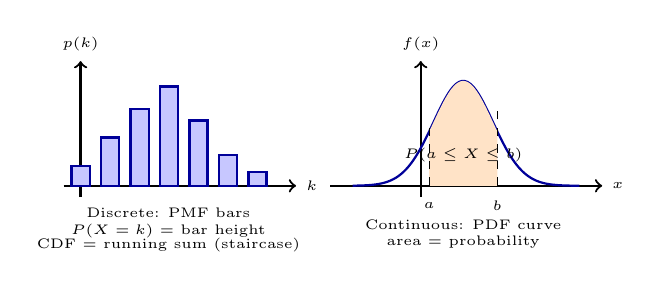
\begin{tikzpicture}[scale=0.72,every node/.style={font=\scriptsize}]
% Left: discrete PMF as bars
\begin{scope}
\draw[->,thick] (-0.3,0)--(3.8,0) node[right,font=\tiny] {$k$};
\draw[->,thick] (0,-0.2)--(0,2.2) node[above,font=\tiny] {$p(k)$};
\foreach \k/\h in {0/0.35,1/0.85,2/1.35,3/1.75,4/1.15,5/0.55,6/0.25} {
  \draw[fill=blue!22,draw=blue!60!black,thick] (\k*0.52-0.16,0) rectangle (\k*0.52+0.16,\h);
}
\node[font=\tiny,align=center] at (1.55,-0.65) {Discrete: PMF bars\\$P(X=k)$ = bar height};
\node[font=\tiny,align=center] at (1.55,-1.05) {CDF = running sum (staircase)};
\end{scope}
% Right: continuous PDF curve
\begin{scope}[xshift=6.0cm]
\draw[->,thick] (-1.6,0)--(3.2,0) node[right,font=\tiny] {$x$};
\draw[->,thick] (0,-0.2)--(0,2.2) node[above,font=\tiny] {$f(x)$};
\draw[thick,blue!60!black,smooth,domain=-1.2:2.8,samples=80] plot (\x,{1.85*exp(-(\x-0.75)*(\x-0.75)/0.55)});
\fill[orange!22] (0.15,0) -- plot[domain=0.15:1.35,samples=40] (\x,{1.85*exp(-(\x-0.75)*(\x-0.75)/0.55)}) -- (1.35,0) -- cycle;
\draw[dashed,thin] (0.15,0)--(0.15,1.05); \draw[dashed,thin] (1.35,0)--(1.35,1.35);
\node[font=\tiny] at (0.75,0.55) {$P(a\le X\le b)$};
\node[font=\tiny] at (0.15,-0.35) {$a$}; \node[font=\tiny] at (1.35,-0.35) {$b$};
\node[font=\tiny,align=center] at (0.75,-0.85) {Continuous: PDF curve\\area = probability};
\end{scope}
\end{tikzpicture}
\caption{Left: discrete PMF (bar heights sum to $1$). Right: continuous PDF (area under curve $=1$; shaded area $=P(a\le X\le b)$).}
\label{fig:pmf-pdf}
\end{figure}

% ============================================================
\section{Bernoulli and Binomial}
\label{sec:bernoulli-binomial}

\begin{definition}[Bernoulli] $X\sim\mathrm{Bernoulli}(p)$ if $P(X=1)=p$, $P(X=0)=1-p$ for $0\le p\le1$. Think: one biased coin toss; $1=$ success.
\end{definition}

\begin{definition}[Binomial] $X\sim\mathrm{Binomial}(n,p)$ if
\[
P(X=k)=\binom{n}{k}p^k(1-p)^{n-k},\quad k=0,\dots,n.
\]
Think: number of successes in $n$ independent $\mathrm{Bernoulli}(p)$ trials.
\end{definition}

\emph{Derivation:} choose which $k$ of $n$ trials succeed ($\binom{n}{k}$ ways), each such pattern has probability $p^k(1-p)^{n-k}$ by independence, sum over patterns (disjoint).

\begin{figure}[h]
\centering
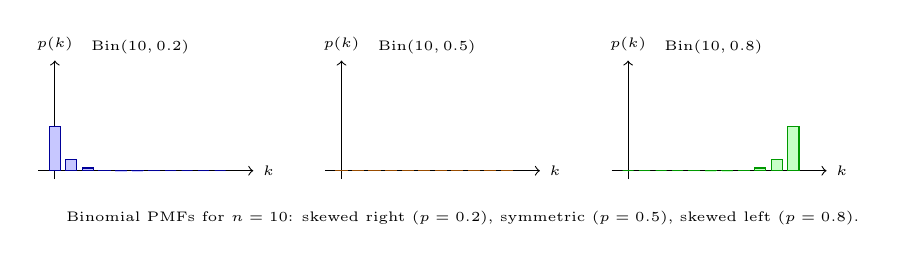
\begin{tikzpicture}[scale=0.70,every node/.style={font=\scriptsize}]
% Three binomial PMFs with different p
\foreach \idx/\p/\col in {0/0.2/blue,1/0.5/orange,2/0.8/green} {
  \begin{scope}[xshift=\idx*5.2cm]
  \draw[->,thin] (-0.3,0)--(3.6,0) node[right,font=\tiny] {$k$};
  \draw[->,thin] (0,-0.15)--(0,2.0) node[above,font=\tiny] {$p(k)$};
  \node[font=\tiny] at (1.55,2.25) {$\mathrm{Bin}(10,\p)$};
  \foreach \k in {0,...,10} {
    \pgfmathsetmacro{\prob}{0}
    % approximate binomial heights: hardcode comb values to avoid divide-by-zero at k=0
    \pgfmathsetmacro{\comb}{1}
    \ifnum\k>0
      \pgfmathparse{1}
      \foreach \j in {1,...,\k} {\pgfmathparse{\pgfmathresult*(10-\j+1)/\j}}
      \pgfmathsetmacro{\comb}{\pgfmathresult}
    \fi
    \pgfmathsetmacro{\prob}{\comb * pow(\p,\k) * pow(1-\p,10-\k)}
    \pgfmathsetmacro{\h}{\prob*7.5}
    \draw[fill=\col!22,draw=\col!60!black] (\k*0.30-0.10,0) rectangle (\k*0.30+0.10,\h);
  }
  \end{scope}
}
\node[font=\tiny,align=center] at (7.4,-0.85) {Binomial PMFs for $n=10$: skewed right ($p=0.2$), symmetric ($p=0.5$), skewed left ($p=0.8$).};
\end{tikzpicture}
\caption{Binomial PMFs $\mathrm{Bin}(10,p)$ for three values of $p$. Shape moves from right-skewed to symmetric to left-skewed.}
\label{fig:binomial-pmfs}
\end{figure}

Mean and variance: if $X\sim\mathrm{Bin}(n,p)$, $\mathbb{E}[X]=np$, $\mathrm{Var}(X)=np(1-p)$ (proved in Ch.~5 via linearity and independence).

% ============================================================
\section{Poisson: Rare Events}
\label{sec:poisson}

\begin{definition}[Poisson] $X\sim\mathrm{Poisson}(\lambda)$ ($\lambda>0$) if
\[
P(X=k)=e^{-\lambda}\frac{\lambda^k}{k!},\quad k=0,1,2,\dots
\]
Think: number of rare events in a large interval when events occur at rate $\lambda$ independently.
\end{definition}

\emph{Why it appears:} $\mathrm{Bin}(n,\lambda/n)\to\mathrm{Poisson}(\lambda)$ as $n\to\infty$ (law of rare events). Use when $n$ large, $p$ small, $np=\lambda$ moderate. Examples: packets arriving at a router per second, typos per page, clicks per minute.

Poisson is \emph{additive}: if $X\sim\mathrm{Pois}(\lambda)$, $Y\sim\mathrm{Pois}(\mu)$ independent, then $X+Y\sim\mathrm{Pois}(\lambda+\mu)$. Mean $=$ variance $=\lambda$.

\begin{example}[Server requests] Requests arrive at $3$/sec on average. $P(\text{exactly }5\text{ in a second})=e^{-3}3^5/5!\approx0.101$. $P(\ge10)$ is the tail $\sum_{k\ge10}e^{-3}3^k/k!\approx0.0011$.
\end{example}

% ============================================================
\section{Normal (Gaussian): The Bell Curve}
\label{sec:normal}

\begin{definition}[Normal] $X\sim\mathcal{N}(\mu,\sigma^2)$ if PDF
\[
f_X(x)=\frac{1}{\sqrt{2\pi\sigma^2}}\exp\!\left(-\frac{(x-\mu)^2}{2\sigma^2}\right),\quad x\in\mathbb{R}.
\]
$\mu$ is the centre, $\sigma$ the spread. Standard Normal $Z\sim\mathcal{N}(0,1)$.
\end{definition}

Key property: \emph{standardisation.} If $X\sim\mathcal{N}(\mu,\sigma^2)$ then $Z=(X-\mu)/\sigma\sim\mathcal{N}(0,1)$. So every Normal probability reduces to the standard CDF $\Phi(z)=P(Z\le z)$ (tabled or via \texttt{erf}).

68--95--99.7 rule: $P(|Z|\le1)\approx0.683$, $P(|Z|\le2)\approx0.954$, $P(|Z|\le3)\approx0.997$.

\begin{figure}[h]
\centering
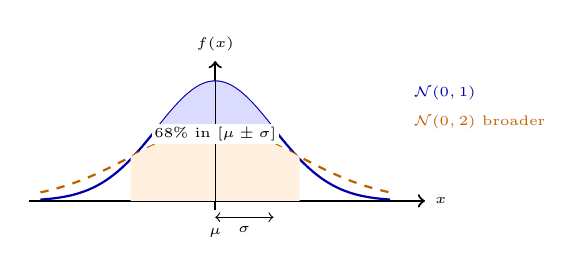
\begin{tikzpicture}[scale=0.74,every node/.style={font=\scriptsize}]
\draw[->,thick] (-3.2,0)--(3.6,0) node[right,font=\tiny] {$x$};
\draw[->,thick] (0,-0.15)--(0,2.4) node[above,font=\tiny] {$f(x)$};
% Normal curves for two sigmas
\draw[thick,blue!65!black,smooth,domain=-3.0:3.0,samples=80] plot (\x,{2.05*exp(-\x*\x/2)});
\draw[thick,orange!75!black,dashed,smooth,domain=-3.0:3.0,samples=80] plot (\x,{1.25*exp(-\x*\x/4.2)});
% 1-sigma shading
\fill[blue!14] (-1,0) -- plot[domain=-1:1,samples=40] (\x,{2.05*exp(-\x*\x/2)}) -- (1,0) -- cycle;
\fill[orange!12] (-1.45,0) -- plot[domain=-1.45:1.45,samples=40] (\x,{1.25*exp(-\x*\x/4.2)}) -- (1.45,0) -- cycle;
% labels
\node[font=\tiny,align=center] at (0,-0.55) {$\mu$};
\draw[thin] (0,0)--(0,2.05);
\node[font=\tiny,fill=white,inner sep=1pt] at (0,1.15) {$68\%$ in $[\mu\pm\sigma]$};
% sigma arrows
\draw[<->,thin] (0,-0.28)--(1,-0.28) node[midway,below,font=\tiny] {$\sigma$};
\node[font=\tiny,anchor=west] at (3.25,1.85) {\color{blue!65!black} $\mathcal{N}(0,1)$};
\node[font=\tiny,anchor=west] at (3.25,1.35) {\color{orange!75!black} $\mathcal{N}(0,2)$ broader};
\end{tikzpicture}
\caption{Normal PDFs: narrow ($\sigma=1$) vs.\ broad ($\sigma\approx1.45$). Shaded $1\sigma$ bands contain $\approx68\%$ of mass. Standardisation maps any $\mathcal{N}(\mu,\sigma^2)$ to $\mathcal{N}(0,1)$.}
\label{fig:normal-pdf}
\end{figure}

\paragraph{Approximations.} For $n$ large: $\mathrm{Bin}(n,p)\approx\mathrm{Pois}(np)$ when $p$ small; $\mathrm{Bin}(n,p)\approx\mathcal{N}(np,np(1-p))$ when $np(1-p)\gg1$ (de Moivre--Laplace / CLT preview). Use continuity correction $P(a\le X\le b)\approx\Phi((b+0.5-\mu)/\sigma)-\Phi((a-0.5-\mu)/\sigma)$.

\paragraph{Other key distributions (used later).} \emph{Geometric} $\mathrm{Geom}(p)$: $P(X=k)=(1-p)^{k-1}p$ ($k\ge1$), trials until first success, $\mathbb{E}=1/p$, memoryless $P(X>m+n\mid X>m)=P(X>n)$. \emph{Exponential} $\mathrm{Exp}(\lambda)$: $f(x)=\lambda e^{-\lambda x}$ ($x\ge0$), continuous analogue of Geometric, also memoryless, models inter-arrival times. \emph{Uniform} $\mathrm{Unif}[a,b]$: constant density $1/(b-a)$. Each appears in Ch.~5--8 for waiting times and random algorithms.

% ============================================================
\section{Computing Distributions in Code}
\label{sec:code-distributions}

\begin{lstlisting}[language=Python]
import math
from math import comb, exp, sqrt, pi, erf

def binom_pmf(n, p, k): return comb(n,k)*p**k*(1-p)**(n-k)
def poisson_pmf(lam, k): return exp(-lam)*lam**k/math.factorial(k)
def normal_pdf(x, mu=0, sigma=1):
    return exp(-0.5*((x-mu)/sigma)**2)/sqrt(2*pi*sigma**2)
def Phi(z): return 0.5*(1+erf(z/sqrt(2)))  # standard Normal CDF

# Examples
print(f"Bin(10,0.3) P(X=3) = {binom_pmf(10,0.3,3):.4f}")
print(f"Pois(3) P(X=5) = {poisson_pmf(3,5):.4f}")
print(f"N(0,1) P(|Z|<=1) = {Phi(1)-Phi(-1):.4f}")  # 0.6827
# Normal approx to Bin(100,0.5): P(45<=X<=55)
mu, sigma = 50, 5
print(f"Normal approx = {Phi((55.5-mu)/sigma)-Phi((44.5-mu)/sigma):.4f}")
\end{lstlisting}

% ============================================================
\section{Chapter Notes}
Bernoulli (1713) and Poisson (1837) distributions are named for their discoverers; Gauss (1809) and de Moivre (1733) shaped the Normal. Knuth TAOCP Vol.~2 covers discrete distributions for random algorithms. The Normal's ubiquity is explained by the Central Limit Theorem (Ch.~6).

% ============================================================
\section{Exercises}
\label{sec:ch04-exercises}
\begin{enumerate}[label=E4.\arabic*, leftmargin=*, itemsep=0.8em]
\item \textbf{Bernoulli to Binomial.} Show from first principles that if $X_i\sim\mathrm{Bernoulli}(p)$ i.i.d.\ then $S_n=\sum_{i=1}^n X_i\sim\mathrm{Bin}(n,p)$. Derive $P(S_n=k)$ by counting outcome strings.
\item \textbf{Poisson additivity.} Let $X\sim\mathrm{Pois}(2)$, $Y\sim\mathrm{Pois}(3)$ independent. Compute $P(X+Y=4)$ two ways: via convolution sum and via $\mathrm{Pois}(5)$. Verify they match numerically.
\item \textbf{Normal standardisation.} $X\sim\mathcal{N}(100,15^2)$ models IQ. Compute $P(X>130)$ and $P(85\le X\le115)$ via $\Phi$. What percentile is $130$?
\item \textbf{Approximation regimes.} For $n=100$, $p=0.02$ ($\lambda=2$), compare $\mathrm{Bin}(100,0.02)$ PMF at $k=0,1,2,3$ with $\mathrm{Pois}(2)$. When does the Normal approximation fail here and why?
\item \textbf{CDF practice.} For $X\sim\mathrm{Bin}(10,0.5)$, compute $F(3)=P(X\le3)$ exactly and via the Normal approximation with continuity correction. What is the absolute error?
\end{enumerate}
% End of Chapter 4
